\documentclass[a4paper,14pt]{article}

\usepackage{comment} % Para comentar várias linhas ao mesmo tempo

%matemática
\usepackage{amsmath}
\usepackage{amssymb}

%diagramação
\usepackage{extsizes}
\everymath{\displaystyle}
\usepackage{geometry}
\usepackage{fancyhdr}
\usepackage{multicol}
\usepackage{graphicx}
\usepackage[brazil]{babel}
\usepackage[shortlabels]{enumitem}
\usepackage{cancel}
\usepackage{textcomp}
\usepackage{tcolorbox}

%tabelas
\usepackage{array} % Para melhor formatação de tabelas
\usepackage{longtable}
\usepackage{booktabs}  % Para linhas horizontais mais bonitas
\usepackage{float}   % Para usar o modificador [H]
\usepackage{caption} % Para usar legendas em tabelas
\usepackage{wrapfig} % Para usar tabelas e figuras flutuantes

\begin{comment}
%tikzpicture
\usepackage{tikz}
\usepackage{scalerel}
\usepackage{pict2e}
\usepackage{tkz-euclide}
\usetikzlibrary{calc}
\usetikzlibrary{patterns,arrows.meta}
\usetikzlibrary{shadows}
\usetikzlibrary{external}
\end{comment}
	
%pgfplots
\usepackage{pgfplots}
\pgfplotsset{compat=newest}
\usepgfplotslibrary{statistics}
\usepgfplotslibrary{fillbetween}

%colours
\usepackage{xcolor}



\columnsep=2cm
\hoffset=0cm
\textwidth=8cm
\setlength{\columnseprule}{.1pt}
\setlength{\columnsep}{2cm}
\renewcommand{\headrulewidth}{0pt}
\geometry{top=1in, bottom=1in, left=0.7in, right=0.5in}

\pagestyle{fancy}
\fancyhf{}
\fancyfoot[C]{\thepage}

\begin{document}
	
	\noindent\textbf{6FMA78 - Matemática} 
	
	\begin{center}Divisão: exercícios (Versão estudante)
	\end{center}
	
	\noindent\textbf{Nome:} \underline{\hspace{10cm}}
	\noindent\textbf{Data:} \underline{\hspace{4cm}}
	
	%\section*{Questões de Matemática}
	
	\begin{multicols}{2}
    	\begin{enumerate}
   			\item Determine o quociente de:
   			\begin{enumerate}[a)]
   				\item 3 : 20 \\\\\\\\\\\\\\
   				\item 15 : 20 \\\\\\\\\\\\\\
   				\item 255 : 30 \\\\\\\\\\\\\\
   				\item 21 : 84 \\\\\\\\\\\\\\\\
   				\item 63 : 15 \\\\\\\\\\\\\\
   				\item 81 : 36 \\\\\\\\\\\\\\
   				\item 13 : 325 \\\\\\\\\\\\\\
   				\item 17 : 340 \\\\\\\\\\\\\\\\\\
   				\item 41 : 20 \\\\\\\\\\\\\\
   				\item 392 : 350 \\\\\\\\\\\\\\
   				\item 414 : 400 \\\\\\\\\\\\\\
   				\item 128 : 125 \\\\\\\\\\\\\\
   			\end{enumerate}
   			\item Calcule.
   			\begin{enumerate}[a)]
   				\item 4,2 : 0,7 \\\\\\\\
   				\item 32,4 : 3,6 \\\\\\\\\\\\\\
   				\item 56,7 : 4,05 \\\\\\\\\\\\\\
   				\item 130,24 : 8,14 \\\\\\\\\\\\\\
   				\item 137,06 : 6,23 \\\\\\\\\\\\\\
   				\item 502,8 : 41,9 \\\\\\\\\\\\\\
   				\item 110,4 : 27,6 \\\\\\\\\\\\\\
   				\item 91,74 : 8,34 \\\\\\\\\\\\\\
   				\item 34,85 : 6,97 \\\\\\\\\\\\\\
   				\item 526,5 : 40,5 \\\\\\\\\\\\\\
   				\item 420,6 : 14,02 \\\\\\\\\\\\\\
   				\item 380,52 : 9,06 \\\\\\\\\\\\\\
   			\end{enumerate}
   			\textbf{Desafio olímpico}
   			(OBMEP) Lucinda manchou com tinta dois algarismos em uma conta que ela tinha feito, como mostra a figura. Qual foi o menor dos algarismos manchados?
   			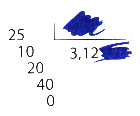
\includegraphics[width=1\linewidth]{6FMA77_imagens/imagem2}
   			\begin{enumerate}[a)]
   				\item 4
   				\item 5
   				\item 6
   				\item 7
   				\item 8
   			\end{enumerate}
   			\item Calcule.
   			\begin{enumerate}[a)]
   				\item 2 : 5 \\\\\\\\\\\\\\
   				\item 13 : 50 \\\\\\\\\\\\\\
   				\item 13 : 4 \\\\\\\\\\\\\\
   				\item 52 : 25 \\\\\\\\\\\\\\
   				\item 87 : 20 \\\\\\\\\\\\\\
   				\item 113,9 : 6,7 \\\\\\\\\\\\\\
   				\item 11,7 : 3,9 \\\\\\\\\\\\\\
   				\item 116,2 : 8,3 \\\\\\\\\\\\\\
   				\item 69,090 : 3,29 \\\\\\\\\\\\\\
   				\item 48,24 : 12,060 \\\\\\\\\\\\\\
   			\end{enumerate}
   		\end{enumerate}
        $~$ \\ $~$ \\ $~$ \\ $~$ \\ $~$ \\ $~$ \\ $~$ \\ 
        \end{multicols}
\end{document}